\documentclass[11pt, oneside]{article}
\usepackage{geometry}
\geometry{letterpaper}
\usepackage{graphicx}
\usepackage{amssymb}
\usepackage{algorithm}
\usepackage{algorithmic}
\usepackage{mathtools}
\usepackage{hyperref}
\usepackage{subfig}
\usepackage{float}
\graphicspath{{../images/}}
\usepackage[backend=biber]{biblatex}
\DeclarePairedDelimiter\ceil{\lceil}{\rceil}
\DeclarePairedDelimiter\floor{\lfloor}{\rfloor}
\usepackage{pgfplots}
\pgfplotsset{width=10cm,compat=1.9}
\addbibresource{planrefs.bib}
\hypersetup{pdfborder=0 0 0}

\begin{document}


\begin{titlepage}
    \begin{center}
        \vspace*{1cm}
            
        \Huge
        \textbf{Adaptive Procedural Generation in Minecraft}
            
        \vspace{0.5cm}
        \LARGE

            
        \vspace{1.5cm}
            
        \textbf{Blake Patterson, Michael Ward}
            
        \vfill
            
            
        \vspace{0.8cm}
            
        
\includegraphics[width=0.2\textwidth]{temple}
            
        \Large
        CIS 5603 Final Project, Dr. Pei Wang \\
        Department of Computer \& Information Sciences\\
        Temple University\\
        May 3, 2022
            
    \end{center}
\end{titlepage}

\pagenumbering{roman}
\newpage
\tableofcontents
\newpage
\pagenumbering{arabic}

\begin{normalsize}

\section{Abstract}
\label{Abstract}

Abstract here

\newpage

\section{Introduction}
\label{Introduction}

	Minecraft is a sandbox video game, created by Mojang in 2009, where players explore and build in a procedurally generated 3D grid-like world with infinite terrain. The main game-play element of Minecraft consists of collecting various types of materials and using them to build tools and structures. The world is divided into 1x1x1 blocks which can vary in material, spawning location, and usability. Aside from the popularity of the base game, Minecraft has become well known for it's customization possibilities through a variety of open source application program interfaces. These application program interfaces allow players to modify textures and color palettes, add new items, block types and enemies, and more. 
	
\begin{figure}[H]%
    \centering
    \subfloat[\centering Grid]{{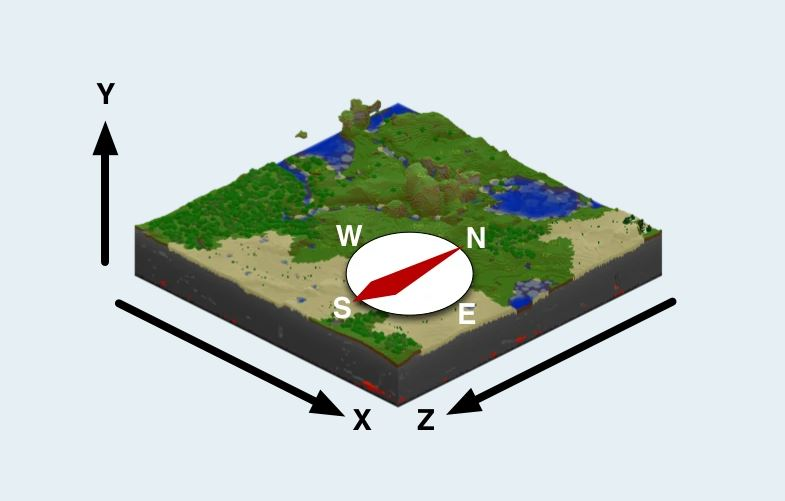
\includegraphics[width=0.4\textwidth]{axis} }}%
    \qquad
    \subfloat[\centering Developer Overlay]{{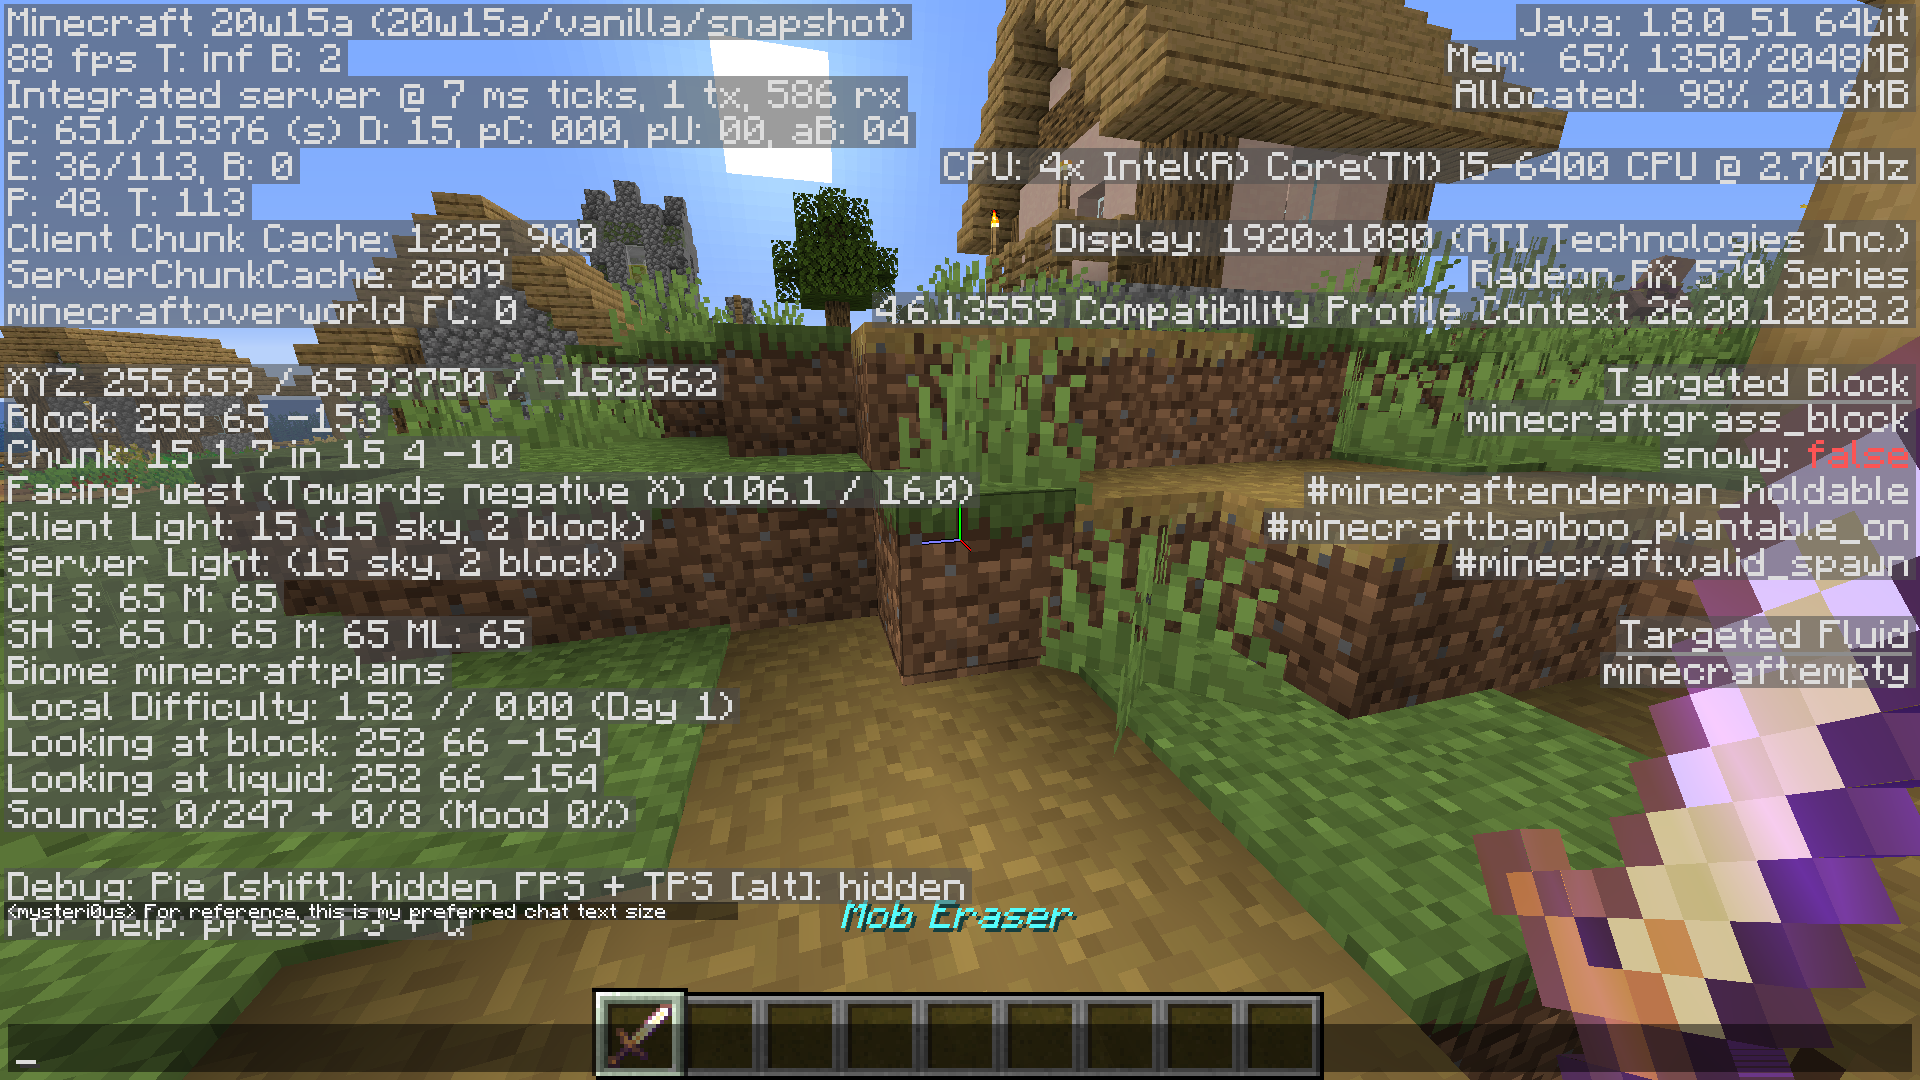
\includegraphics[width=0.5\textwidth]{f3} }}%
    \caption{Observable Minecraft Environment}%
    \label{fig:env}%
\end{figure}

The open source nature and in-game environment of Minecraft has also caught the attention of artificial intelligence researchers. The environment of Minecraft is ideal for research in AI because of the endless possibilities, from training an agent on simple tasks like searching for a specific object or material, to building complex structures or navigating obstacle courses. Since the environment is divided into a three-dimensional grid of equal sized cubes, it is also easy to measure and evaluate the performance of AI in Minecraft.

This project is focused on the application of AI for Procedural Content Generation (PCG) within Minecraft. PCG is defined as the algorithmic creation of game content with limited or indirect user input \cite{shaker2016procedural}. Content in the context of PCG can be described as most of what can be contained within a game including maps, rules, textures, items, quests, music, characters, and more \cite{shaker2016procedural}. Many popular games have made use of PCG including Rogue, Dwarf Fortress, Diablo, Spore, Civilization, Spelunky, as well as Minecraft itself \cite{shaker2016procedural}. The usage of PCG varies from game to game and can range from fully autonomous game design, to  automating routine or common aspects of game design. One major critique of PCG in game design has to do with repetition and functionality; rule-based agents are likely to create good looking and functional content that looks similar, and search-based agents are likely to create more diverse content, but takes more time and resources to ensure that it is functional for the player \cite{green_organic_2019}.

Most instances of PCG in video games operate from a 'clean-state' where the generator does not have to consider interaction with preexisting in-game elements \cite{green_organic_2019}. Exploring PCG within Minecraft opens up a new challenge within AI, in which the goal is to produce a functional and believable village settlement that adapts to different environments within a Minecraft map \cite{salge_generative_2019}. Instead of generating a village on a clean slate, this problem restricts the generator with the presence of preexisting game elements and focuses on adaptive generation of artifacts \cite{green_organic_2019}. A map in Minecraft is made up of various biomes which contain different types of terrain, elevation gradients, fauna, and bodies of water. In order for a procedurally generated settlement to be functional and believable, it must be adaptive and able to build on top of and in response to elements that already exist in the Minecraft environment. The Generative Design in Minecraft Competition (GDMC) AI settlement generation competition initially proposed this problem in 2018 \cite{salge_generative_2018}. GMDC has ran a yearly open competition for researchers and students to submit their algorithm, which is scored by a panel in terms of the algorithms adaptability and functionality \cite{fridh_settlement_nodate}. 

We propose to develop a Procedural Content Generation AI that is capable of generating a functional and believable Minecraft settlement, which is adaptive to varying environmental factors. Based on our review of literature, it is apparent that developing multiple different algorithms to handle individual pieces of the problem has led to better outcomes in previous research. 

\newpage

\section{Related Work}
\label{Related Work}

\subsection{PCG in Games}

The most common use of Procedural Content Generation (PCG) in video games historically has been dungeon generation. Dungeons are labyrinthine-like environments which are made up of intricate pathways leading to rewards, puzzles, or progression points \cite{van2013procedural}. Surveys on the use of PCG for dungeon generation found that it has been applied mostly to 2D games, while rarely being found used in 3D games \cite{viana2019survey}. These same surveys found that two main approaches have been used for PCG, constructive algorithms and search-based algorithms. Constructive algorithms are usually based on random positioning, cellular automata, or graphs grammars. 

\subsubsection{Constructive Algorithms}
Cellular automata applies a set of rules for specifying cell-state transitions based on cells' neighbors to a two dimension grid of cells \cite{adams2017procedural}. This method repeatedly applies the defined set of rules to the grid, which leads to the change of cell states until the grid stabilizes. Cellular automata methods for PCG generates large 2D maze-like patterns, which are generally merged using a region merging algorithm to ensure that the entire area is playable \cite{adams2017procedural}. This approach is generally used in PCG to create a randomized spatial structure / layout for a level or dungeon. See figure \ref{fig:dungeon} (a) for an example of a map generated with cellular automata.

\begin{figure}[H]%
    \centering
    \subfloat[\centering Map generated with ceullar automata. Grey areas represent floor, red represents walls, and white represents rocks \cite{johnson2010cellular}]{{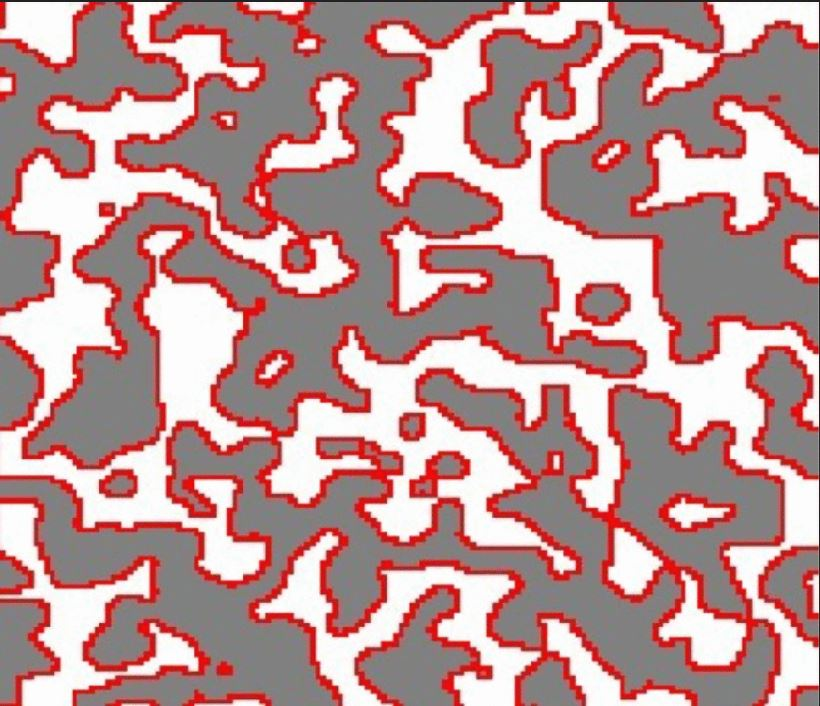
\includegraphics[width=0.3\textwidth]{cells} }}%
    \qquad
    \subfloat[\centering (a) mission with tasks, keys, and locks. (b) mission structure from (a) mapped spatially. (c) gameplay graph (d) dungeon layout generated by (c) \cite{van2013procedural}]{{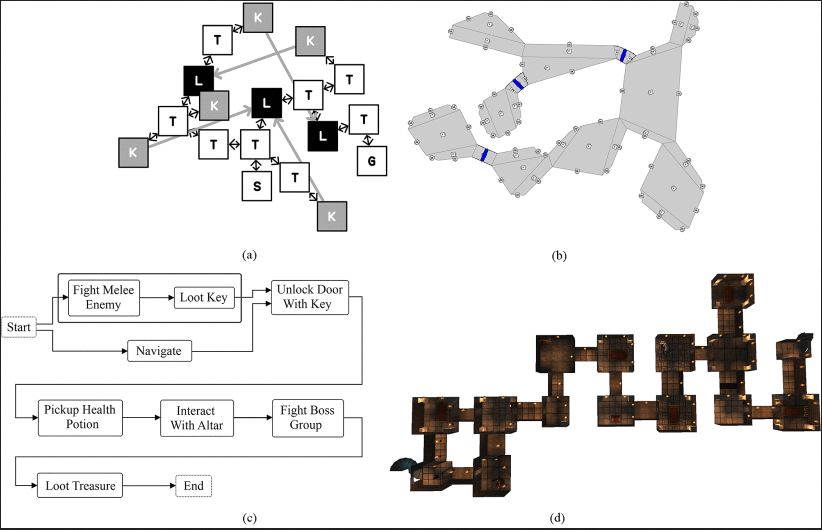
\includegraphics[width=0.5\textwidth]{graphs} }}%
    \caption{Dungeon Methods}%
    \label{fig:dungeon}%
\end{figure}

Graph grammar is an extension of generative grammar, a system of grammatical rules used to generate sentences or words \cite{thompson2017generative}. Graph grammar is used in PCG to support the creation of levels that are divided into rooms. Typically, player actions are mapped onto a directed graph, which is then used to generate the dungeon or level layout. Nodes on the graph are the player actions, while graph edges indicate the order of actions. This procedure works well for dungeon or level based games because typically, the geometry and content of a level are dependent on gameplay requirements, not the other way around \cite{van2013designing}. See figure \ref{fig:dungeon} (b) for examples of gameplay graphs and their generated layouts.

Overall, constructive PCG algorithms present solutions for 3D games, and only one in recent times supported adaptive generation \cite{viana2019survey}. So while this work is relevant and informative to our work, we did not opt to use these approaches in the current iteration of our project.

\subsubsection{Search-based Algorithms}

One form of search-based algorithm that has appeared in PCG is genetic algorithms \cite{togelius2011search}. In general, genetic algorithms encode possible solutions to an optimization problem into strings, which are then evaluated by a fitness function. The genetic algorithm then goes through an iterative process of calculating the fitness of solutions then selecting \& combining solutions into new strings. A survey of genetic algorithms in PCG found this type of algorithm applied in multiple fashions.

One such approach uses genetic algorithms to generate a game world that allows linear progression, using a list of plot points and locations of known types as input \cite{hartsook2011toward}. This approach represents genotypes as a tree data structure where each node represents a portion of the game environment, see figure \ref{fig:gen} (a). It also represents designer-specified probability for two environment types to be adjacent to each other using an environment transition graph (see figure \ref{fig:gen} (b)). Generations that more closely match the environment transition graph score highly, while those that diverge from the graph score lower. The fitness function that this approach uses measures average bridge length, average \# of sidepaths, average \# of sidepaths per bridge, total \# of sidepaths, total \# of nodes, environment transition probability, and environment transition variance (bridges are areas of the world where non-plot-specific game play occurs).

\begin{figure}[H]%
    \centering
    \subfloat[\centering Genetic Space Tree \cite{hartsook2011toward}]{{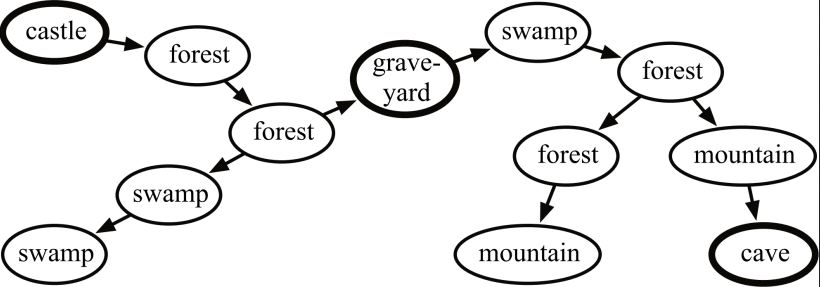
\includegraphics[width=0.4\textwidth]{gen1} }}%
    \qquad
    \subfloat[\centering Environment Transition Graph \cite{hartsook2011toward}]{{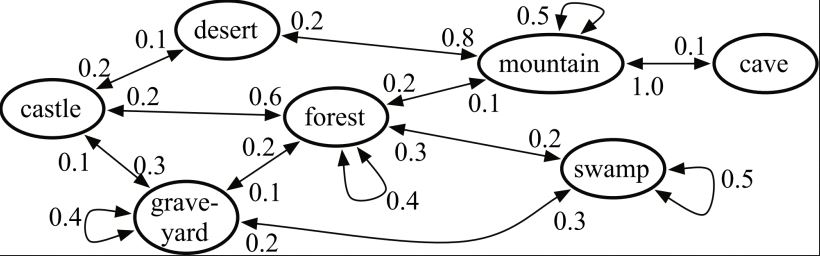
\includegraphics[width=0.4\textwidth]{gen2} }}%
    \caption{Genetic Tree Representations}%
    \label{fig:gen}%
\end{figure}

This specific implementation of genetic algorithm applied to PCG is geared towards 2D role playing games, but the authors believe that it could be applied to any other story-oriented game. We did not end up applying any genetic algorithms in our approach, but did make use of a modified fitness function for our plot analysis algorithm.

\subsubsection{Architectural PCG}

PCG for architecture has been used in video games, as well as general digital media. One recent approach to PCG for architecture uses a declarative (easily steered to intended typology) and comprehensive (capable of creating multiple typologies) tile-based generator \cite{van2020declarative}. This method makes use of architectural profiles (also called tile profiles), which are a semantic segmentation that characterizes different types of architectural building blocks. These architectural profiles are then combined, using adjacency conditions that are applied to each type of architectural profile. A tile solver translates the adjacency conditions into logic constraints, which then determines tile placement. Examples of tile profiles and their tile adjacency semantics can be seen in figure \ref{fig:tile}. This method is capable of producing a large range of architectural styles, in terms of density (ratio of interior and exterior space) and repetitiveness (prevalence of patterns in terms of tile placements). 

We have not gotten far enough in our current project iteration to tackle building interiors, but this approach looks promising for creating adaptive building interiors \& exteriors in Minecraft. The authors of this work comment that while this approach is game agnostic, they believe it has potential for generating urban environments in Minecraft \cite{van2020declarative}. 

\begin{figure}[H]%
    \centering
    \subfloat[\centering Tile profiles. From left to right, first row (interior tiles): corner, wall, door, window, interior area; second row (exterior tiles): roof, street, stairs, landing, void tile. \cite{van2020declarative}]{{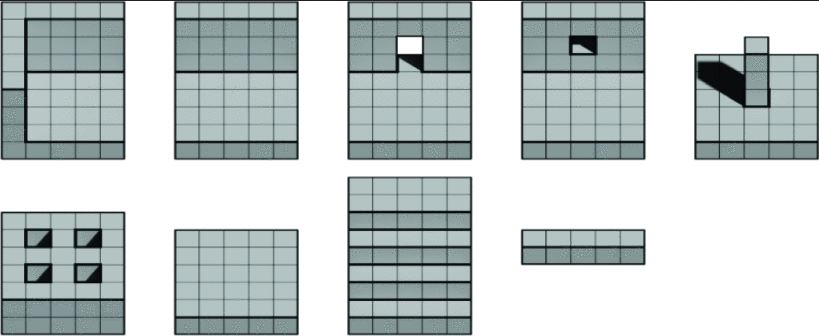
\includegraphics[width=0.5\textwidth]{tiles}}}%
    \qquad
    \subfloat[\centering Semantics on tile adjacency conditions, in two types: traversal (in red) and construction (in yellow). \cite{van2020declarative}]{{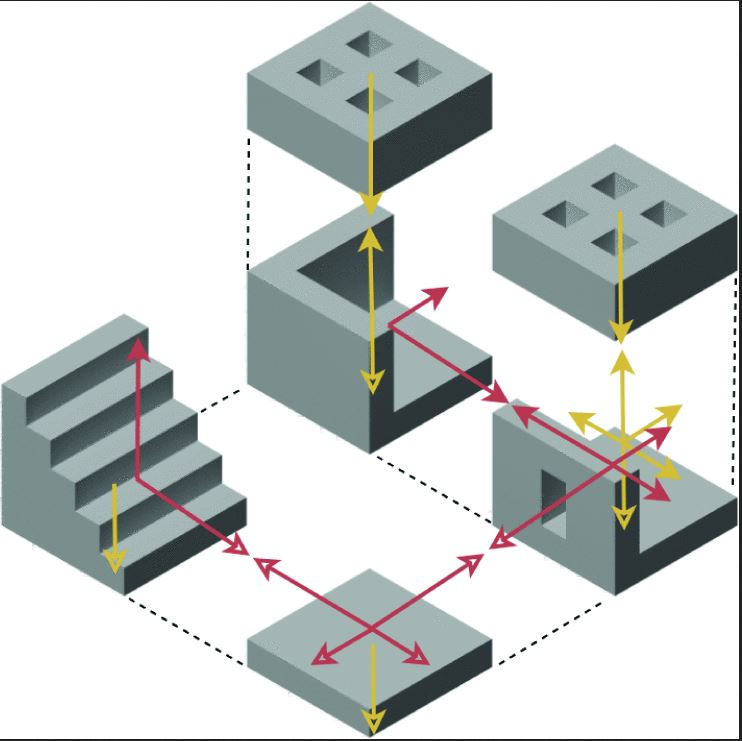
\includegraphics[width=0.3\textwidth]{tile_mix} }}%
    \caption{Architecture Methods}%
    \label{fig:tile}%
\end{figure}

\subsubsection{Reinforcement Learning in PCG}

While reinforcement learning has been used to teach an agent how to play a game many times, using it to teach an agent how to generate a game level has not been explored to the same extent \cite{khalifa2020pcgrl}. This particular application of reinforcement learning has not appeared in literature until 2020. Khalifa et al. speculate that the reason for it's absence is that it's unclear how to approach the level generation process as a reinforcement learning problem.

To frame this problem as a RL problem, the authors describe PCG as an iterative task rather than generating all content in one step, which allows them to model PCG as a markov decision process. To represent the level generation problem as a MDP, they used three different representations of the state space, action space, and transition function that are taken from earlier RL approaches. In the first representation which they call 'Narrow', the agent is restricted to a predetermined sequence of build locations. In the second representation which they call 'Turtle', agents have control over their current location, but only with respect to their last location. Lastly, in the third representation which they coined as 'Wide', the agent has full control over location and tile type. They applied these three agents to three different 2D level generation problems. To illustrate how their approach works, we'll describe one of the problems. In the 'Zelda' problem, the level must have exactly one player, one door, and one key, and the player must be able to reach the key and the door in a set number of steps. The level may have enemies, which cannot spawn within a certain radius of the player. The goal of the agent in this scenario is to modify the 2D level \cite{khalifa2020pcgrl}.

Ultimately the authors found that the agent struggled to design complex levels, but was still able to generate a large number of playable levels. This approach isn't easily mappable to the broad topic of village generation in Minecraft, but is a unique recent approach to PCG in game design. We aren't sure of how easily this methodology could be broadly extended to 3D games, but if possible, then player created villages could be used as the training materials. This approach could, however, potentially be applied to the specific problem in our work of generating building floorplans, since a Minecraft building floorplan can be easily flattened to a 2D space.


\subsection{PCG in Minecraft}

As described in the introduction, many different AI approaches have been implemented in Minecraft. In this section we will describe a few of the most closely related recent papers to our topic of settlement generation in Minecraft.

\subsubsection{GDMC}

\paragraph{Competition Description}

One of the existing research areas that piqued our interest in this topic is the Generative Design in Minecraft Competition. This competition encourages AI researchers to produce AI agents that are capable of generating functional, aesthetically appealing, and believable villages / settlements that adapt to a randomly selected location in Minecraft \cite{salge_ai_2020},\cite{salge_generative_2018},\cite{salge_generative_2019}. The competition evaluates submissions based on adaptability, functionality, believable narrative, and visual aesthetics. Adaptability measures how well structures adapt to terrain, whether structures reflect the surrounding environment, and whether the settlement takes advantage of terrain or compensates with terrain issues. Functionality measures how accessible the settlement is for players, whether there is easy access to resources such as food and water, whether it scales well as size increases, and whether there are protections from danger. Believable narrative measures how well the settlement tells a story, shows how it was developed, evokes a narrative, and whether there's a sense of culture. Visual aesthetics are a measure of how good the settlement looks (subjective), whether there is a consistent look to the settlement, and whether there is an appropriate level of variation \cite{salge_ai_2020}. While the GDMC competition was our initial inspiration for this project, we are not set on submitting to the competition at this stage in the project. We did lean on several of the more concrete evaluation metrics of the competition when developing our methods, particularly adaptability and functionality.

The GDMC competition has been a yearly occurrence since 2018, but unfortunately few competitors have released papers discussing their approach and methodology, aside from a yearly summary report that's put out by the official competition. It started with just 4 competitors in 2018, and has risen to 20 by 2021, with many of the teams returning each year to submit their improved versions. We have found a detailed paper that applies a multi-agent approach in 2021's competition, as well as a cellular automata approach taken in 2019's competition.

\paragraph{Competition Submissions}

Esko and Fritiofsson developed a multi-agent system for PCG in Minecraft for the 2021 GDMC competition \cite{esko2021multi}. This approach differs from approaches we've seen implemented in code that lack a written report - it is the only approach so far that's implemented a multi-agent system where all generative tasks are performed by an agent in real time, via a NPC (non-player character). The generator sequence described by this approach scans and abstracts the selected build area, creates a founding seed, generates the roads and then lastly generates buildings. Similarly to our approach, the authors generated a height map of the area (see figure \ref{fig:height} on page \pageref{fig:height} for a height map example), as well as a liquid map. We did not use a liquid map in our implementation - they created it by taking the height map, and checking the block above for water, and setting the array value at that position to 1 if water is found, and 0 if no water is found. They used the combination of these two maps to create a weighted directed graph where each node represents a coordinate from the height map, and the weight of the edges is dependent on the height difference between nodes \cite{esko2021multi}. This approach builds the settlement by expanding from a center point, which they refer to as a founding seed. They do several depth-first searches of the height map and liquid map to identify regions of similar height, discarding nodes that differ too much from the average. This algorithm determines a starting location with the most space to grow the settlement. Once the founding seed has been identified, they utilize two sets of agents deemed 'extendor agents' and 'connector agents'. Extendor agents are tasked with extending the road network - they perform random walks over the terrain within the initial given build area. When the agent discovers a node not currently part of the road network, they use Djikstra's algorithm to find the closest piece of road to connect it to. Connector agents are tasked with increasing the connectivity of the road network, ensuring that any two points in the settlement have direct routes. These agents use a Digital Differential Algorithm to make sure that road intersection opportunities are not missed. This algorithm runs every time the agent takes a step, and draws lines in random directions to determine if any other roads are within a given range. Once the roads have been created, a plotting agent also performs random walks to determine suitable building locations. Once an agent finds a location that isn't road and not overlapping an existing plot, it performs bounded depth-first search to expand the plot to a certain boundary, which is then built upon \cite{esko2021multi}. The biggest difference between this approach and our chosen approach (aside from use of multiple agents) is that this paper builds roads before building plots, and uses Djikstra's algorithm instead of A\* algorithm for road building.

One other methodology paper exists alongside a GDMC submission, which details an approach to generating floor plans using cellular automata algorithms. This paper by Green et al. summarizes their approach to both floor plan generation and external wall generation \cite{green_organic_2019}. They use a constrained growth algorithm to generate each building's floor plan, which grows in single block steps. First, they determine the number of rooms by taking the rounded cubed root of the total building area, which they have restricted to a rectangular shape. Each room is given a random initial starting location, which is always 2 x 2, then the rooms take turns growing one block at each step until none of the rooms can grow any larger. Doors are then placed with certain restrictions based on the placement of rooms. Once the internals of the house are complete, the external walls are generated using a neighbor summation algorithm taken from cellular automata. This algorithm doesn't care about the states of specific neighbors at each cell, but rather the sum of those states. In this example, state 0 is a solid block, and state 1 is a glass window block. They wanted to achieve a ratio of 75\% solid blocks and 25\% glass windows, so they made the rules for cellular automata that if the sum of neighbors is 2 or 3, the current block is set to be glass, otherwise it is set to be a solid block. This approach leads to randomized, but functional walls that lead to a nice variety of looks for buildings. The authors comment that the modularity of this approach also allows for customization later on, if they want to swap in a different method for one of the steps, such as a grammar based approach \cite{green_organic_2019}. Overall, this approach to generating floor plans and walls checks all the boxes that we are focusing on, namely functionality and adaptability, and is an approach that we are considering for our floor plan design when we reach that point.


\subsubsection{Related Minecraft PCG}

There are two other non-GDMC AI approaches in Minecraft that are relevant to our work and worth discussing. The first approach is a project called World-GAN, which uses generative adversarial networks to generate arbitrarily sized world chunks from a small sample size \cite{awiszus2021world}. While many researchers have explored graph grammar and rule-based algorithms for PCG in games, this project is one of few papers we found in our research area that uses Machine Learning techniques for PCG in games, and the only one using Machine Learning for PCG in Minecraft. This project contributes a 3D GAN architecture for PCG in Minecraft, and uses a block2vec technique that is inspired by word2vec. The training pipeline for WorldGAN can be seen in figure \ref{fig:gan}. They tested this approach on biomes in Minecraft, and were able to sucessfully change the styles of one biome to another (i.e. change the style of a generated forest biome to a desert biome).  

\begin{figure}[H]
\centering
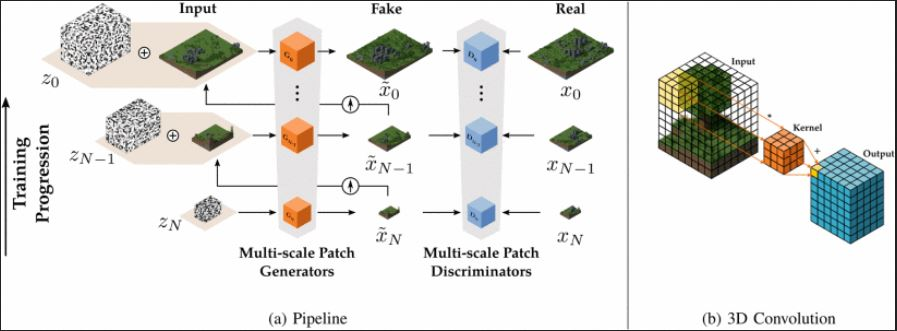
\includegraphics[width=0.9\textwidth]{gan}
\caption{World-GAN training pipeline \cite{awiszus2021world}}
\label{fig:gan}
\end{figure}

This approach is very interesting, but for our desired use it didn't seem like the correct fit. This approach is very good for altering the biome in a given area, but is not able to transfer structures. It would be possible to train the GAN on a sample that contains houses and other structures, but there isn't any type of semantic enforcement of 'structural correctness' within the current methodology. The authors confirm that models trained on samples containing structures result in non-functional and non-sensical structures. While we chose not to pursue this methodology, this is a project to keep an eye on, as the authors commented their interest in GDMC and plans to continue researching this topic.

The last related approach we'd like to discuss is another cellular automata based methodology. While other researchers we've mentioned have explored the use of cellular automata for level generation and floorplan generation, Sudhakaran et al. have developed a Neural Cellular Automata (NCA) model which is capable of generating entire structures in Minecraft \cite{sudhakaran2021growing}. This model is capable of higher dimensionality than similar previous work (3D vs 2D),  capable of using more types of constructive units than previous models, and capable of evaluating all surrounding cells of a given cell using 3D convolutions, compared to just four immediate neighbors. The model works by training on target structures, then generating copies of the target structures over a series of epochs. Overall, this model is capable of generating small structures quickly and with high accuracy, but struggles with larger structures - taking large amounts of time and encountering random artifacts \cite{sudhakaran2021growing}. This approach was also interesting, but not easily applicable to our problem. Down the road an approach like this seems like it could be useful for generating buildings, but it would require training on many different sizes and styles of buildings in order to be used adaptively.


\section{Methodology}
\label{Methodology}

\subsection{Interface Mod and Python Client}

We chose to implement our various algorithms \& methodologies using Python, but we still needed some way of communicating with Minecraft. 
To do this we chose to make use of the Generative Design in Minecraft Challenge (GDMC) HTTP Interface Mod and corresponding Generative Design Python Client (GDPC). 
As mentioned before, GDMC is a yearly competition for researchers and students to submit their procedural generation algorithms for Minecraft. 
In order to allow competitors to focus more on the algorithms themselves as well as to foster more consistency between how the submissions communicated with Minecraft, some members of GDMC developed these tools \& made them open source for all to use. 

The GDMC HTTP Interface Mod, is, as it sounds, a mod for Minecraft. 
A Minecraft mod, or modification, is a user made piece of additional software that adds onto the core source code of Minecraft. 
Countless mods exist for Minecraft, most of which are for the purpose of enhancing the game's performance/visuals or adding new content to the game, but many functional mods such as this interface mod also exist. 
In order to make additional software work with Minecraft, however, an API needs to be in place that will make Minecraft recognize and properly implement the mod's code (since Minecraft's code itself is closed \& not directly modifiable).
The most popular of which is Minecraft Forge, so we had to set up Forge for our machines. 
With Forge set up, we simply installed the GDMC HTTP Interface Mod and that was that. 

The mod itself does one simple yet vital thing within Minecraft: whenever a world is opened a corresponding HTTP server is launched on localhost port 9000. 
Thus, with the mod set up on our machines, as long as we had a Minecraft world open, we could communicate to it through this HTTP server via basic HTTP requests to certain endpoints. 
For example, if we wanted to know what block was at a certain (x, y, z) coordinate in the world, we could make a GET request to the server at the blocks endpoint (i.e., "localhost:9000/blocks") with the coordinates as parameters and it would return information about the block at those coordinates. 
On the other side of things, if we wanted to place a block, we could perform the same request but as a PUT rather than GET request as well as provide a block ID as a parameter, and the corresponding block would be placed at those coordinates in the world. 
There are multiple other endpoints which serve multiple other purposes, all of which can be found in the GDMC documentation. 

Technically the mod alone is enough for us to communicate with Minecraft, although having to write the HTTP requests ourselves is tedious. 
Luckily the mod's developers also thought of this and created the GDPC, which we will refer to simply as the Python client, to alleviate this tediousness. 
The Python client is a framework strictly to be used alongside the GDMC HTTP Interface Mod in order to make sending the necessary HTTP requests much easier. 
It can essentially be thought of as a wrapper, which allows us to simply call functions to communicate with Minecraft rather than write the HTTP requests ourselves. 
For example, rather than writing GET \& PUT requests to get \& place blocks manually, the Python client defines two functions to do exactly that, getBlock \& placeBlock. 
It even goes beyond the basic operations and defines functions such as placeCuboid \& placeCenteredCylinder to make building larger more involved structures easier. 
The Python client also makes obtaining information about the world substantially easier. 
For example, in one line of code the Python client allows us to obtain a world slice, which, in short, contains all of the information about a certain section of the Minecraft world that we could ever need \& puts it in a nicely packaged data structure for us. 
The rest of the functionality provided by the Python client can again be found in the GDMC documentation, however, the functionality described here is largely all that was needed for this project. 


\subsection{Terraforming}

When testing our program, we quickly encountered an issue specific to Minecraft for this type of procedural village generation, trees. Trees in Minecraft can appear in almost any biome, \& can be densely populated or sparsely populated. Trying to place a building on an patch of land that already contains trees leads to various undesirable results, as seen in figure \ref{fig:tree}. Building on top of preexisting trees can lead to houses being filled with trees, trees poking out the tops of houses, \& sometimes even houses being placed on top of trees. Since our goal is to build a settlement in any randomized location within Minecraft, handling the presence of trees is a key factor of an adaptable village generator.

This problem of adapting to existing structures is one unique to our project. As discussed previously, procedural content generation most typically operates on a clean slate. Since this problem is somewhat unique to our project, there is not an accepted methodology for handling preexisting tree structures. While this is a problem that any teams who submit or have submitted work to the GDMC competition would have to address, few teams have produced written work detailing their methodology.

To solve this problem, we used our knowledge of trees \& the data structures that are accessible via the Python client to devise an algorithm that can efficiently locate \& remove trees that are present in a randomly selected build area. Trees in Minecraft have the same attributes as real-life trees; they grow straight up from the ground, are made of wood, \& typically have leaves surrounding the canopy. Trees in Minecraft are made specifically from wood blocks, which are solely found in the form of trees. With this knowledge, we could create an algorithm that searches the 3-dimensional space until it finds a wood block, then searches the y-coordinate space up \& down from that block until wood isn't found any more in either direction. This was our first approach, but it was computationally expensive. The typical build area size we tested on is 128 x 128 x 128 blocks, so at worst this algorithm would explore roughly 2 million blocks. To come up with a more efficient algorithm, we needed to find a better way to search the 3D space -  this was quite difficult as there is no maximum number or minimum number of trees in any given x,y,z boundaries within Minecraft. 

\begin{figure}[H]%
    \centering
    \subfloat[\centering Trees in house]{{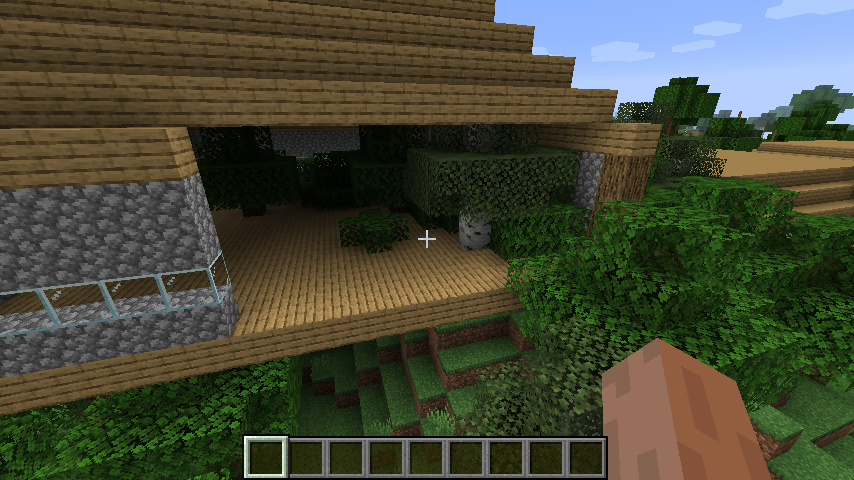
\includegraphics[width=0.4\textwidth]{tree1} }}%
    \qquad
    \subfloat[\centering Trees on house]{{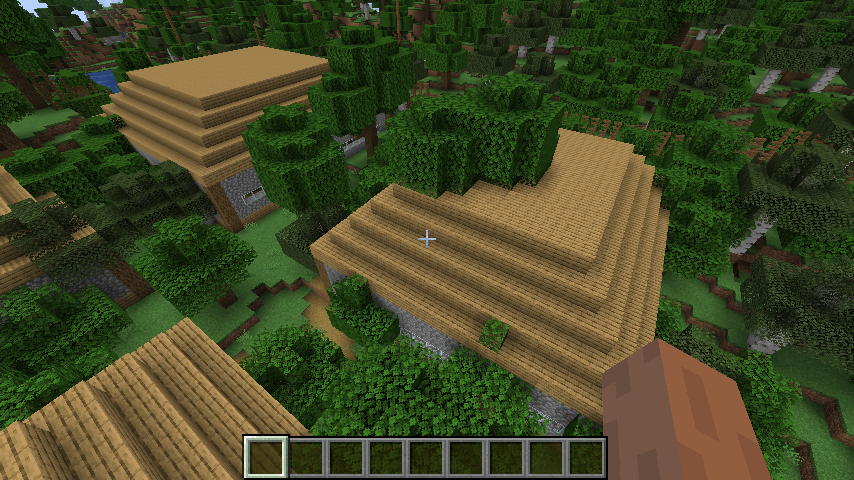
\includegraphics[width=0.4\textwidth]{tree2} }}%
    \caption{Building on trees examples}%
    \label{fig:tree}%
\end{figure}

In order to restrict the search space, we extracted a height map of the given build area using the GDMC Python client - which is a 2D array the size of the the x,z coordinate space that contains the highest y coordinate value (not containing air or leaves) at each x,z coordinate combination. See figure \ref{fig:height} for an example of a height map for an 8 x 8 area. Instead of searching potentially the entire 3D space, we could search the 2D height map for the presence of wood blocks instead, which would give us a starting node for each tree - the top block of each tree. Since the height map is the highest y coordinate in each x,z coordinate combination, we can assume that any given coordinate in a height map is the top of a tree if the coordinate contains a wood block.

Once the height map has been searched for the presence of wood blocks, the 3D space can be searched, using the tree top coordinates obtained from the height map search as starting nodes. Each node is expanded downwards until wood blocks are not found, giving us the full coordinate map of trees in the build area. An inverted conical buffer is applied to each tree's coordinate space to ensure the removal of leaves, and then the tree coordinates and buffer space are replaced with blank space. This search algorithm is much more efficient than the first search algorithm used, \& at worst searches roughly 16,000 blocks in a 128 x 128 x 128 build area.

\begin{figure}[H]
\centering
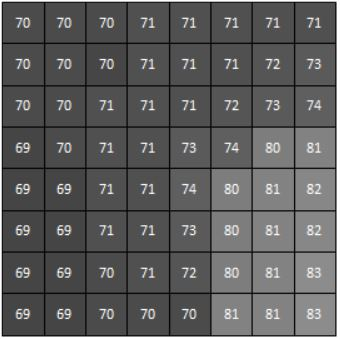
\includegraphics[width=0.3\textwidth]{height}
\caption{Example of an 8 x 8 heightmap \cite{esko2021multi}}
\label{fig:height}
\end{figure}

\subsection{Plot Analysis}

After clearing the designated build area of trees, it was necessary to compute how buildings and structures should be distributed across the build area. The distribution of buildings is a key piece of the problem that we want to solve, which is determining how a procedurally generated village should adapt to various randomly selected terrain. For this problem we also applied a search-based approach, using a fitness/evaluation function which grades the suitability of different locations in the build area for the purpose of house building.

Our plot analysis algorithm divides the randomly selected build area into subdivisions that are based on the size of the total build area. For each subdivision, it generates a height map \& calculates the standard deviation of height within each respective subdivision. From here, the fitness function uses the standard deviations of height to evaluate which subdivisions are suitable for building houses on, with a preference for locations with low standard deviation of heights.

This algorithm could be further improved by adding additional vectors to the fitness function. Some vectors which we think could be useful to include are the percentage of water present in subdivision \& distance to the nearest body of water from subdivision centroid. These vectors could help the fitness function to avoid building in areas with small patches of water \& also be set to build either near or far from water sources such as rivers or ponds. Another problem that our current algorithm runs into is that sometimes it will unnaturally place one building far away from the main grouping of buildings - this can happen if there's a hill that has a small flat area on top of it, while the rest of the area is relatively flat. This could be solved by calculating the height gradient of the entire build area \& tuning the fitness function to prefer placing buildings in the same gradient of the build area.

\subsection{House Building}

With land cleared \& plot locations determined, the next step was to build a structure at each plot. 
To start off we chose to implement arguably the most common structure in Minecraft, something that is a must for any settlement, a house. 
There are different methods out there that other researchers have developed which make use of various AI techniques to build a house which changes based on different factors, but as our focus was more on the settlement as a whole and making the layout adapt to the land around it, we chose to implement a basic house building procedure. 
This allowed us to put more time into plot analysis \& path building, which were both more important to our overall goal than each individual house. 

In the end, we developed one main function which takes in six parameters: a set of starting x, y, \& z coordinates, and a set of ending x, y, \& z coordinates. 
The starting x \& z coordinates determine the bottom left most point of the house \& the ending x \& z coordinates determine the top right most point of the house. 
The starting y coordinate determines floor level \& the ending y coordinate determines ceiling level (this does not account for the roof, which goes about five blocks above ceiling level).
With these parameters set up \& some predetermined materials in place (i.e., oak planks for the floor, cobblestone for the wall, etc.), the function iterates through the different dimensions, placing the floor \& some support pillars, followed by the walls \& windows, followed by the roof, and finishes off with a door. 

Finally. as one last step, we added one supplementary function on top of the main house building function. 
This function takes in an array of coordinates to build houses at (i.e., the result of our plot analysis) and calls the build house function with a slight random adjustment to each of the parameters. 
This not only made sense from a code organization perspective, but allowed us to add some random naturalness to our houses rather than have them be all the same size. 

\subsection{Path Building}

With the all of the houses placed, our settlement is nearly completely built, save for one final piece: the paths. 
Every settlement has paths connecting the different structures, even in real life, so we had to come up with a methodology to generate paths between each of our structures in a natural looking yet still functional way. 
The immediate choice that comes to mind, which also turned out to be the best choice for our situation, was A*.  

This is not the place to be reviewing the exact details of what A* is, but in short it is a state space searching technique popular in the field of AI. 
The reason it is popular within AI, and considered an AI technique itself, is because it takes into account the cost of the path (i.e., $cost(p)$) as well as a heuristic evaluation of the path (i.e., $h(p)$), rather than simply calculating the exact optimal path outright. 
This means we had to determine how to evaluate the cost of our path so far as well as how to heuristically evaluate it in such a way that led to a natural looking yet functional path within Minecraft. 
As it turns out, the most typical cost \& heuristic functions used in standard grid search problems worked incredibly well in Minecraft. 
In short, the cost function was simply equal to how many blocks the path had stretched so far, and the heuristic function was equal to the Manhattan distance from the end of the path to the goal destination.
More specifically, we calculated the Manhattan distance as $|x' - x| + |z' - z|$, where $(x, z)$ are the coordinates for the end of the current path \& $(x', z')$ are the coordinates for the goal destination.
One might understandably ask why the vertical y coordinate is excluded, and the simple answer is that the resulting paths were better without it. 
This is most likely because we did not ultimately want to traverse vertically all that often, and all that really mattered was the horizontal traversal of the path. 

With the cost \& heuristic functions set up, there is only one thing left to determine: the boundaries of our path. 
More specifically, where can A* look when determining where to place the path, or even more accurately, where can it not look? 
This is where our implementation of A* had to become slightly modified from most. 
See, most implementations of A* are concerned with two dimensional grids/planes of some sort, and they do not have to worry about a third, vertical dimension. 
Simply ignoring the third dimension would not work though, as if we ran it normally it would lead to massive, immediate vertical jumps in the path which not only do not look natural, but are also non-functional. 
Also, simply restricting the path to only work in two dimensions is not only does not make sense theoretically since the player is entirely capable of moving vertically, but almost never works in practice since the land in Minecraft is rarely perfectly flat. 
Thus, this led us to determine that the path should be able to move vertically, but only by one block at a time because any more and the player would not be able to traverse it. 
This, unsurprisingly, worked very well and led to natural looking \& functional paths. 

There was still one problem, however, and that was the horizontal boundaries at which A* was able to place paths. 
If A* is unable to reach its destination in a relatively direct way, it will start trying increasingly indirect ways to reach its destination. 
In fact, by default, it will exhaustively search the entire possible set of paths within the grid it is searching to determine if there is a possible path. 
This does not work in Minecraft, however, because the world of Minecraft is, for all intensive purposes, infinitely large. 
Thus, if there was no immediate direct path, or even a relatively indirect one, A* would continue for as long as possible before terminating. 
Not only did this lead to ridiculously long run times, but it also led to extremely inefficient paths. 
To solve this, we simply put in a restriction that said A* cannot go outside a certain border that was predefined along with the settlement itself. 
If it was not possible to reach the destination within these boundaries it would simply place the best path it could before terminating. 

With all of these parameters \& rules in place, we simply had A* run and then place a chunk of blocks at each point along its determined path (as one block did not look natural enough). 
Then, we set up a simple function which took in the coordinates of the front of each house \& built paths between each of the houses such that everything was interconnected. 
All said \& done, this implementation of A* led to relatively natural looking \& functional paths. 

\section{Discussion}
\label{Discussion}

\subsection{Results}

In the end, we were able to implement everything as described in the previous section within the allocated time frame. 
There were definite issues faced during the implementation and not everything worked perfectly in the end, but that will be discussed later. 
First off, let us examine two settlements generated from our program. 

Here is a settlement generated on relatively flat terrain in a dense forest. 
\begin{figure}[H]
    \centering
    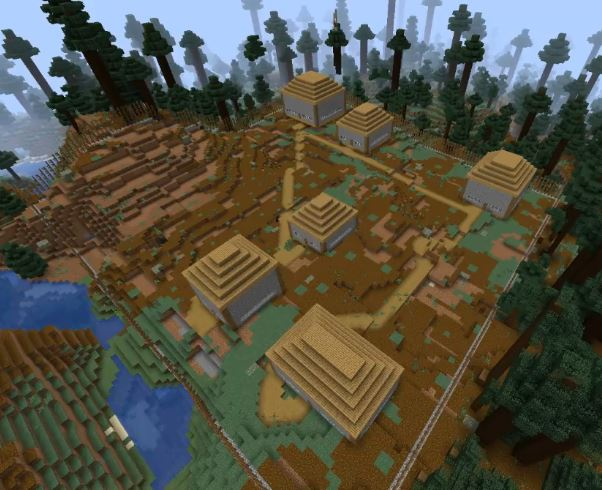
\includegraphics[width=0.75\linewidth]{village1}
    \caption{Flat Dense Forest Settlement}
    \label{fig:env}
\end{figure}

There are multiple noteworthy aspects of this first settlement that can be taken away \& examined. 
First of all, it is clear to see that the terraforming methodology worked perfectly. 
The area in which the settlement was built (marked by the perimeter fence) was completely cleared of trees. 
The next thing worth noting is the house placement. 
This is much more subtle, but the plots at which the houses were placed make sense.
Notice how no house was placed near the hill towards the left of the image. That is because it would not make sense to place a house on hilly terrain, and our program handled that as intended. 
The next step of our program was building the houses, and there is not much to talk about here aside from the fact that the houses were built as expected. 
Finally, we can take note of the paths. 
In terms of hard requirements for a usable path, the paths our program generated meet all of them. 
They reach the front door of every house, they are relatively flat, and they are efficient (i.e., they generally take the most direct path possible). 
On top of that, the paths also look natural. 
If you asked a random player if they thought another player built these paths, it would be reasonable of them to say yes, and that was what we were aiming for. 

Next, here is a settlement generated on much more uneven land near a mountain \& river. 
\begin{figure}[H]
    \centering
    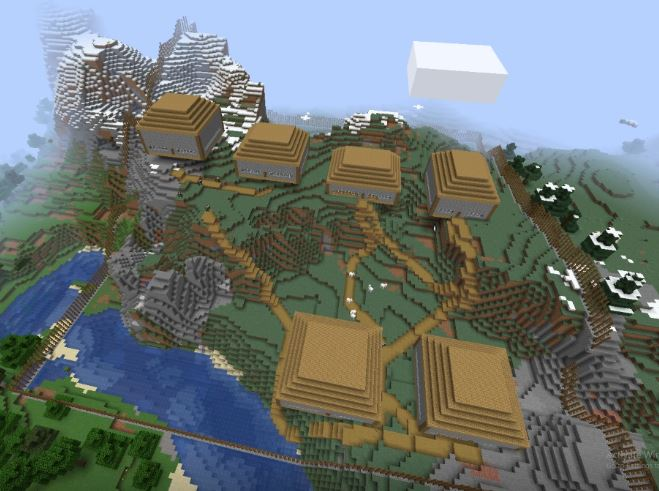
\includegraphics[width=0.75\linewidth]{village2}
    \caption{Mountainous River Village}
    \label{fig:env}
\end{figure}

This environment is clearly a much tougher one to build a settlement in, so let us examine how the same aspects from the previous settlement were handled in this one. 
First off, terraforming was less of an issue here, but as you can see, it was still handled perfectly as there are no trees in the build area. 
Secondly, the house placement was probably the biggest issue here. 
It is almost impossible to perfectly place houses on this piece of land without completely tearing the land apart, so our program did the best it could to pick relatively flat pieces of land to place the houses. 
With that in mind, the program did fairly well. 
It did not place any houses on the river, it did not place any houses in the middle strip of land which was too hilly, and it did not place any houses in the far back piece of land which was far too hilly. 
Moving onto the houses themselves, they were again built exactly as expected, so let us examine the paths. 
This piece of land was much more of a test for our path methodology as it is far more hilly, but, as you can see, our program generated fairly natural looking \& functional paths yet again. 
The paths clearly navigate the hills relatively easily, which is what we were aiming for with our implementation of A*. 
There are two notable problems, however, and those are that one of the paths did not finish (in the top left of the image), and some of the paths reached the house but were multiple blocks below the front door of the house (making the house inaccessible). 

\subsection{Issues \& Limitations}

Having seen the results of our final program, let us examine the issues \& limitations faced along the way. 
First we will start by discussing issues with the interface mod \& Python client, then move on to issues with our implementation of plot analysis \& how it connects with house building, and finally finish with issues regarding our implementation of path building. 
Terraforming \& house building were implemented using simple yet fairly efficient \& accurate techniques, so there is not much to be discussed there (aside from how they could be improved, which will be discussed in next steps).

The first major issue we faced had to do with the nature of the framework we used to communicate with Minecraft, the interface mod \& Python client. 
As described earlier in this paper, this framework allows us to communicate with Minecraft through the use of HTTP requests (i.e., if we wanted to place a block in the world, we have to send a corresponding HTTP request for that to happen). 
This is all great \& works perfectly in moderation, but it does not scale well as you start to perform more \& more operations. 
More specifically, when we were just testing out the framework and building small structures like simple small houses, there were no issues. 
However, as we progressed to building entire settlements containing multiple houses, it required many more HTTP requests to be sent back to back. 
This led to one major problem: when too many HTTP requests were sent back to back, many of them would just be dropped leading to the corresponding operation not being completed. 
In short, this meant that builds would just look incomplete (i.e., some trees would not be fully destroyed, there would be holes in some of the houses, etc.).
The natural solution for most developers would just be to make the requests synchronous and if one returned with a bad or incomplete status, just repeat it. 
We would agree, and we would have done this had we written the requests ourselves, but the Python client is not directly editable and does not handle the requests in this way. 
In fact, the Python client does not directly allow for callbacks in any sense, you simply call a function such as placeBlock and hope it works. 
Considering the Python client worked perfectly in every other aspect \& writing our own requests would be a fairly large task, we decided to go with a more temporary solution: simply making as few requests as possible and blocking the program very briefly between large batches of requests. 
This solved the problem to a sufficient enough degree for us to finish, but if we were to have more time it would be ideal for us to write our own framework for sending the HTTP requests.

Moving on, we will point out all notable issues with our implementation of plot analysis \& how it connects with house building. 
The first notable issue is the lack of randomness \& naturalness to the plots. 
More specifically, if run in the same area twice (or just run on perfectly flat land multiple times), it will pick the same pieces of land to put houses on. 
This is obviously not an issue for pieces of land where there are only so many places to naturally put a house (like in the examples above), but on flat land this leads to "suburban" looking houses (i.e., houses lined up in a row \& column type layout). 
Ideally, we would most likely add a hint of randomness to make the house placements look more natural in environments where houses could viably be placed anywhere, but seeing as our implementation handled natural, hilly environments very well it was not a big issue. 
Another issue we faced had to do with when there were no pieces of flat land large enough to place a house on. 
More specifically, the issue was our lack of handling this. 
In its current version, our implementation will simply aim to put the houses on the flattest land possible, even if that land is not actually flat relative to the player. 
Then, it would simply build the house on top of the highest point of that land. 
If the part of the land in front of the door was lower than the highest point, then this would lead to the door being too high off the ground (as can be seen in the examples above). 
On the other hand, if the land in front of the door was the highest point and the other land was lower, it would look like the house was only supported in the front (which is unnatural looking). 
Ideally, we would have fixed this by having an additional terraforming step which further flattened plots which needed it. 
Lastly, our house building methodology simply needed to be more diverse \& random. 
At the moment, our program often led to nearly identical houses, all facing the same way. 
This is not a huge issue \& has nothing to do with our main goal of adapting to the land as naturally as possible, but it is simply not very appealing. 

Finally, we will discuss all notable issues with our implementation of path building. 
The most notable issue has to do with the order of the paths. 
To be more specific, the way each path is placed in the current version of this project is that the program connects house 1 \& 2, then 2 \& 3, then 3 \& 4, and so on. 
This often times leads to fairly natural and efficient looking paths, so it is not an issue most of the time. 
However, the problem is that sometimes it leads to interweaving networks of paths that do not look natural and simply do not make sense from a functional perspective. 
Ideally, the paths should not just directly go between each house, but connect to each additional path in the most natural way possible. 
Additionally, it should be possible for there to be a center point or intersection for the paths where ever it would make sense. 
The next issue with our paths, which is much less noticeable in any of the settlements generated, has to do with the lack of terraforming. 
More specifically, sometimes it would just make more sense to simply destroy or place some blocks in the land when there is a vertical gap rather than try and go around it. 
The main limitation we faced regarding this was not knowing when it was better to destroy or place a block rather than going around, so we did not get to implementing this. 
The only other main issue we had regarding path building was the possible search space for a path and how to handle when no possible path was found. 
Regarding the search space, it was hard to determine what was too big and what was too small. 
Too big and you would almost always find a possible path, but the run time would be terrible as it might try an absurd number of possibilities before picking a path (even after implementing the most efficient tie breaking method for A*).
Too small and, while the run time would not be bad, it might not find a possible path even if there was one obvious to the player. 
To solve this, the current version of the program simply uses the build area (marked by the perimeter fence) as the boundaries to the path builder, although this still led to issues on occasion. 
Regarding when a possible path is not found, we chose to simply build the final state A* was in after terminating, but this led to wildly inefficient paths.  
This is because our implementation of A* will not always necessarily terminate on the closest to optimal path it found if it could not find a complete path.
Luckily this did not occur all too often with our boundaries set to the entire build area, although it is still an issue in the current version.  

\subsection{Next Steps}

1. add randomness to plot analysis

2. additional terraforming step to flatten plots before placing houses

3. smart house building 

4. more structure to our paths / smart path placement

5. deep neural networks

6. more structures 


\section{Acknowledgments}
\label{Acknowledgments}

We'd like to thank the contributors and maintainers of both the \href{https://github.com/nilsgawlik/gdmc_http_interface}{Minecraft HTTP Interface Mod} and \href{https://github.com/nilsgawlik/gdmc_http_client_python}{Generative Design Python Client}: Nils Gawlik, Claus Aranha, Mayank Jain, and Flashing-Blinkenlights. This project would not be possible without the tools they built that allow for interacting with Minecraft via Python scripts.

\newpage

\section{References}
\label{references}
\nocite{*}
\printbibliography[heading=none]

\end{normalsize}
\end{document}